\subsection{Advanced Sampling}
Comparison plot, including methods from the previous week. (1000 experiments)
\begin{center}
    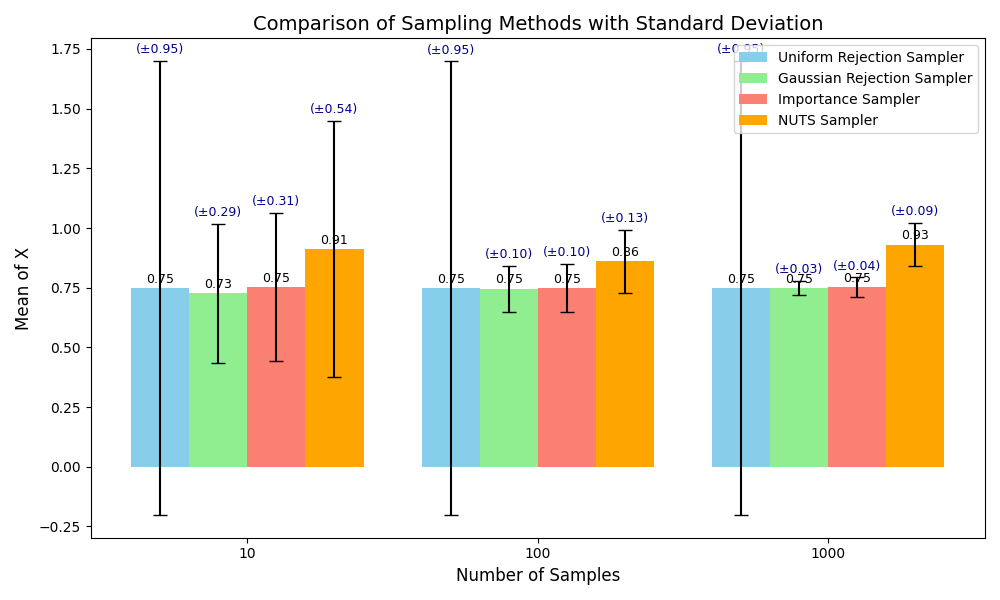
\includegraphics[width=12cm]{./figures/comparison2.png}
\end{center}
From this comparison we can notice that the Nuts sampler is consistently overestimating the target mean, unlike the simpler methods.
In terms of variance NUTS only beats the uniform rejection sampler.
The Nuts samplers variance scales well with the number of samples, 
although it trails behind the Gaussian rejection and importance samplers variances.





\subsection{Programming GPs}

The code is shown in~\cref{sec:week4:code:gp}.

A plot showing samples from a Gaussian Process
with mean $m(x) = 0$ and kernel
$k(x, y) = \exp{\left( -\gamma \parallel x - y \parallel^2 \right)}$
with $\gamma = 10$.
is shown in~\cref{fig:week4:gp:gp-samples}.

For predicting the CO2 levels at Mauna Loa, Hawaii,
we followed the template and used the ``special kernel'',
using grid search to find optimal parameters.
The optimal parameters were
\begin{align*}
  \sigma_y &= 0.1155\ldots \\
  \eta_1 &= 0.1112 \\
  \eta_2 &= 8.8889.
\end{align*}
The mean and 95\% confidence interval of the posterior,
along with the training data and true measurements,
is shown in~\cref{fig:week4:gp:predict},

\begin{figure}[htbp]
  \centering
  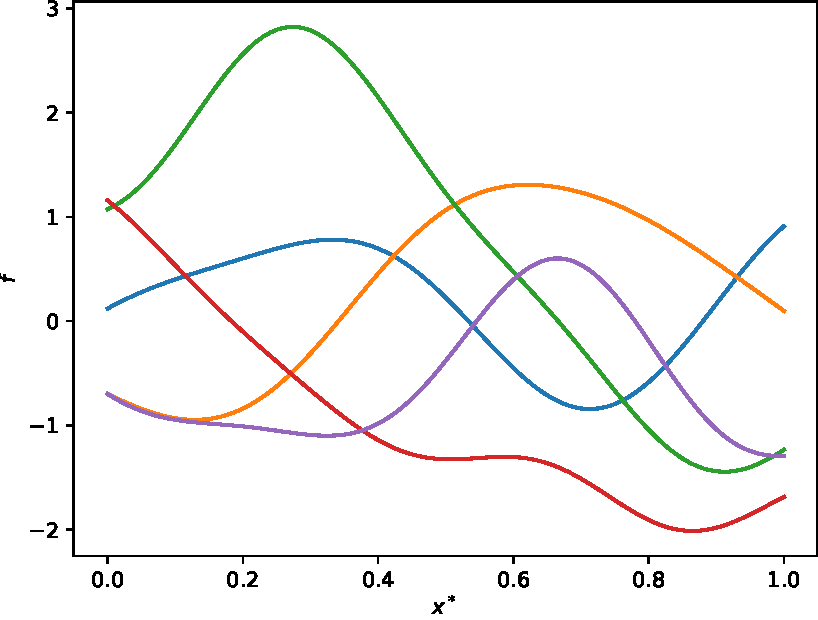
\includegraphics[width=0.7\textwidth]{./figures/gp_samples.pdf}
  \caption{Samples from a Gaussian Process with a Gaussian kernel.}
  \label{fig:week4:gp:gp-samples}
\end{figure}

\begin{figure}[htbp]
  \centering
  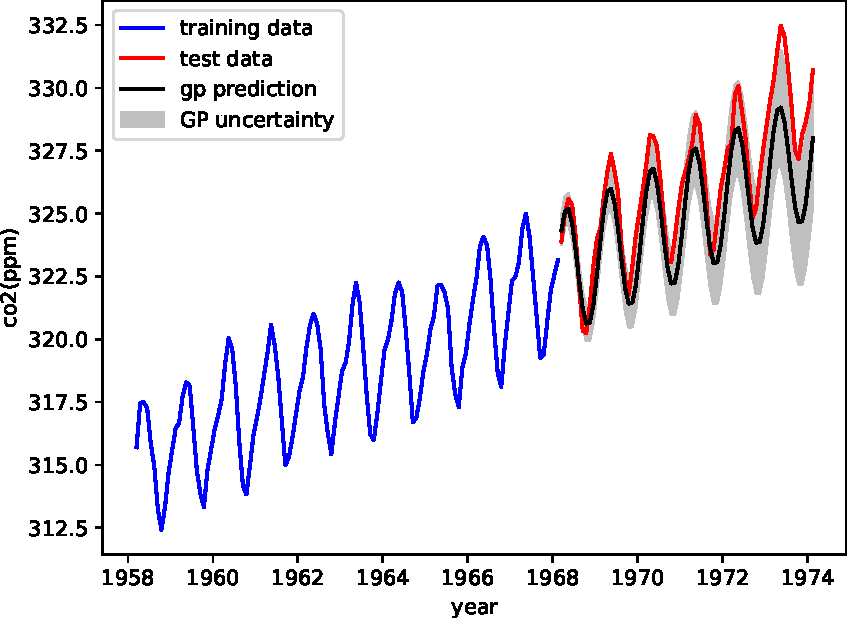
\includegraphics[width=0.8\textwidth]{./figures/gp_predict.pdf}
  \caption{
    Posterior $p(f^\ast | x^\ast, \mathcal{D})$ trained on
    CO2 measurements at Mauna Loa, Hawaii.
    The black line shows the mean $\mu^\ast$ for $x^\ast$,
    and the gray region marks the 95\% confidence interval,
    $\mu^\ast \pm 1.96 \sigma^\ast$.
  }
  \label{fig:week4:gp:predict}
\end{figure}
